\documentclass{standalone}
\usepackage{tikz}
\usetikzlibrary{arrows,shapes,positioning,shadows,trees}

\begin{document}
\begin{tikzpicture}
  \node(z) at (0,0) {
    \begin{tikzpicture}
      \draw (0,0) circle (1);
      \node[fill,circle,inner sep=1pt,label=below:$O$] at (0,0) {};
    \end{tikzpicture}
  };

  \node(f) at (z.east) [anchor=west, xshift=0.3cm] {
    \begin{tikzpicture}
      \draw[->] (0,0) -- (2,0);
      \node[anchor=south] at (1,0) {$f$};
    \end{tikzpicture}
  };

  \node(f_z) at (f.east) [anchor=west, xshift=0.3cm] {
    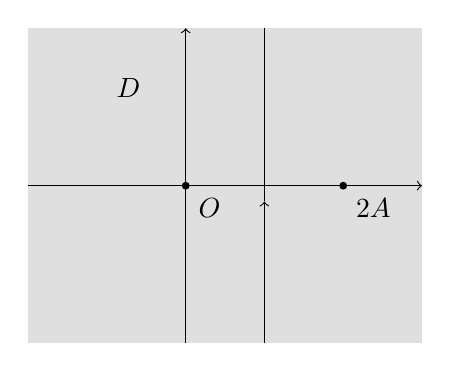
\begin{tikzpicture}
      \fill[gray!50,opacity=0.5] (-2,-2) rectangle (3,2);
      \draw[->] (-2,0) -- (3,0);
      \draw[->] (0,-2) -- (0,2);
      \node[fill,circle,inner sep=1pt,label=below right:$O$] at (0,0) {};
      \node[anchor=south west] at (-1,1) {$D$};
      \node[fill,circle,inner sep=1pt,label=below right:$2A$] at (2,0) {};
      \draw[->] (1,-2) -- (1,-0.2);
      \draw[-] (1,-0.2) -- (1,2);
    \end{tikzpicture}
  };

  \node(phi) at (f_z.south) [anchor=north, yshift=-0.3cm] {
    \begin{tikzpicture}
      \draw[->] (0,0) -- (0,-2);
      \node[anchor=west] at (0,-1) {$\phi$};
    \end{tikzpicture}
  };

  \node(phi_f_z) at (phi.south) [anchor=north, yshift=-0.3cm] {
    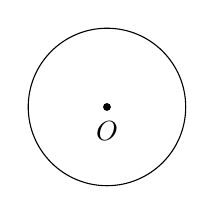
\begin{tikzpicture}
      \draw (0,0) circle (1);
      \node[fill,circle,inner sep=1pt,label=below:$O$] at (0,0) {};
    \end{tikzpicture}
  };
  \draw[->] (z) -- (phi_f_z);
\end{tikzpicture}
\end{document}